\section{数据可视化案例:豆瓣电影Top 250}

在之前的介绍中,我们大致认识了Power BI Deskto的界面和基本生成图表的操作。接下来,我们将通过一个数据可视化分析的实际案例,来完整地体验和了解Power BI的强大功能。

本节将对豆瓣电影Top 250网页上的数据进行数据可视化并生成报告作为主要案例。网页如\figref{fig:douban_movie_main_page}所示。

\begin{figure}[htbp]
    \centering
    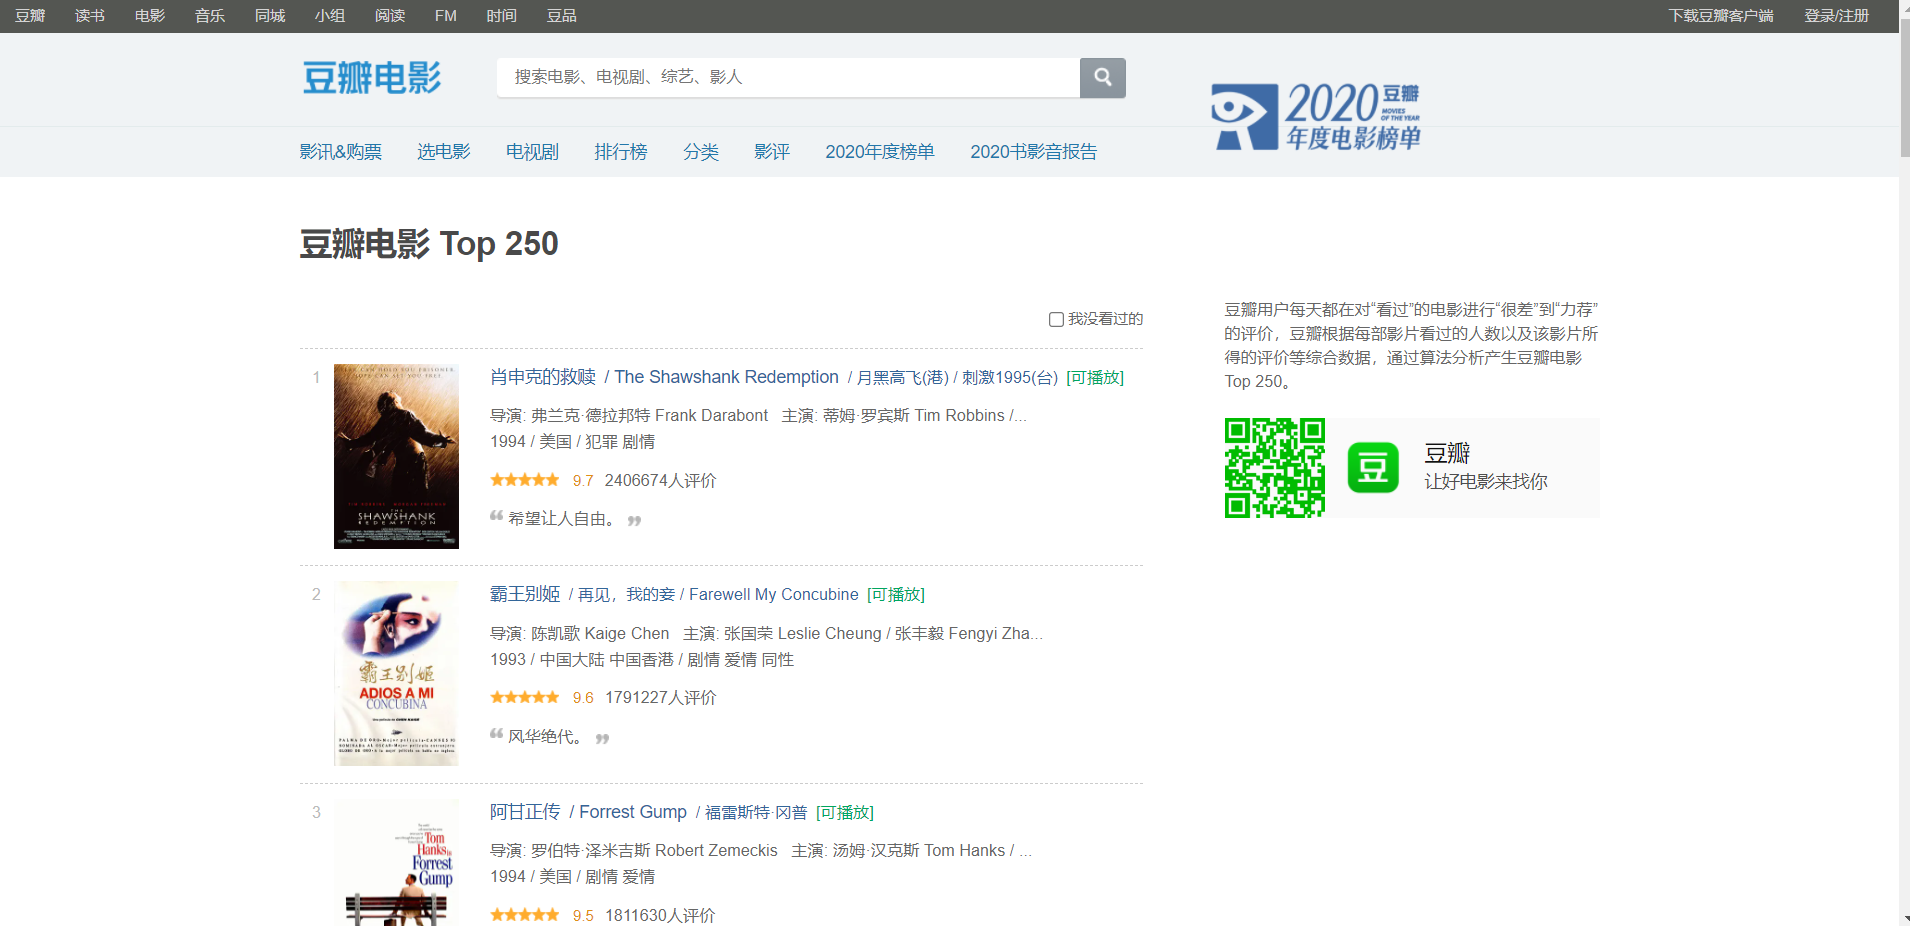
\includegraphics[width=0.9\textwidth]{figure/PowerBI/douban_movie_main_page.png}
    \caption{\textbf{豆瓣电影Top 250主页}}
    \label{fig:douban_movie_main_page}
\end{figure}

我们将利用Power BI抓取豆瓣电影Top 250的电影数据,经过数据清洗、数据建模并形成一个可视化报告,该报告分为4页的报表,含有封面页和数据页,以便更清晰地查看和理解Top 250的电影信息,如中所示。

% TODO

下面开始介绍实现过程。

\subsection{数据准备和处理}

数据分析的第一步是获取数据,在Power BI中,支持了上百种数据格式和数据来源,Excel、MySQL、Spark、Web等几乎用户所能接触到的数据形式都有广泛良好的支持。此处即为对Web网页数据的抓取。

\subsubsection{分析网页结构}

打开豆瓣电影Top 250网页(地址:\url{https://movie.douban.com/top250})发现每页仅显示25部电影,Top 250共分为了10个网页。通过点击不同的页数,可观察到每一页的网址的规律:\url{?start=25}为第2页,\url{?start=50}为第3页……各页是通过最后的?start=的参数来控制的。熟悉该规律后,便可进行批量提取全部10页的数据。

\subsubsection{提取第1页数据}

打开Power BI Desktop,单击``获取数据''组中的``Web'',如\figref{fig:douban_import_from_web}所示。

\begin{figure}[htbp]
    \centering
    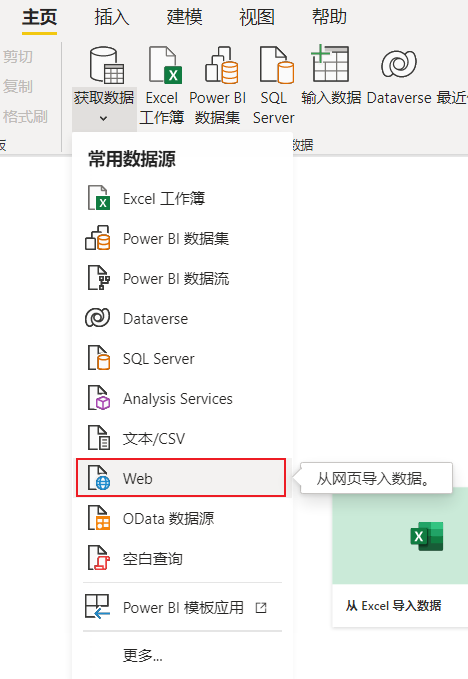
\includegraphics[width=0.4\textwidth]{figure/PowerBI/douban_import_from_web.png}
    \caption{\textbf{从Web获取数据}}
    \label{fig:douban_import_from_web}
\end{figure}

在弹出的窗口中输入第1页的网址:\url{https://movie.douban.com/top250?start=0},点击``确定'',并``连接''。

等待建立连接后,在弹出的导航器中,如\figref{fig:douban_advice_table}所示,在``建议的表格''里,Power BI已自动地识别出了每一部电影的各个信息,包含了电影名、评分、描述、导演等。

\begin{figure}[htbp]
    \centering
    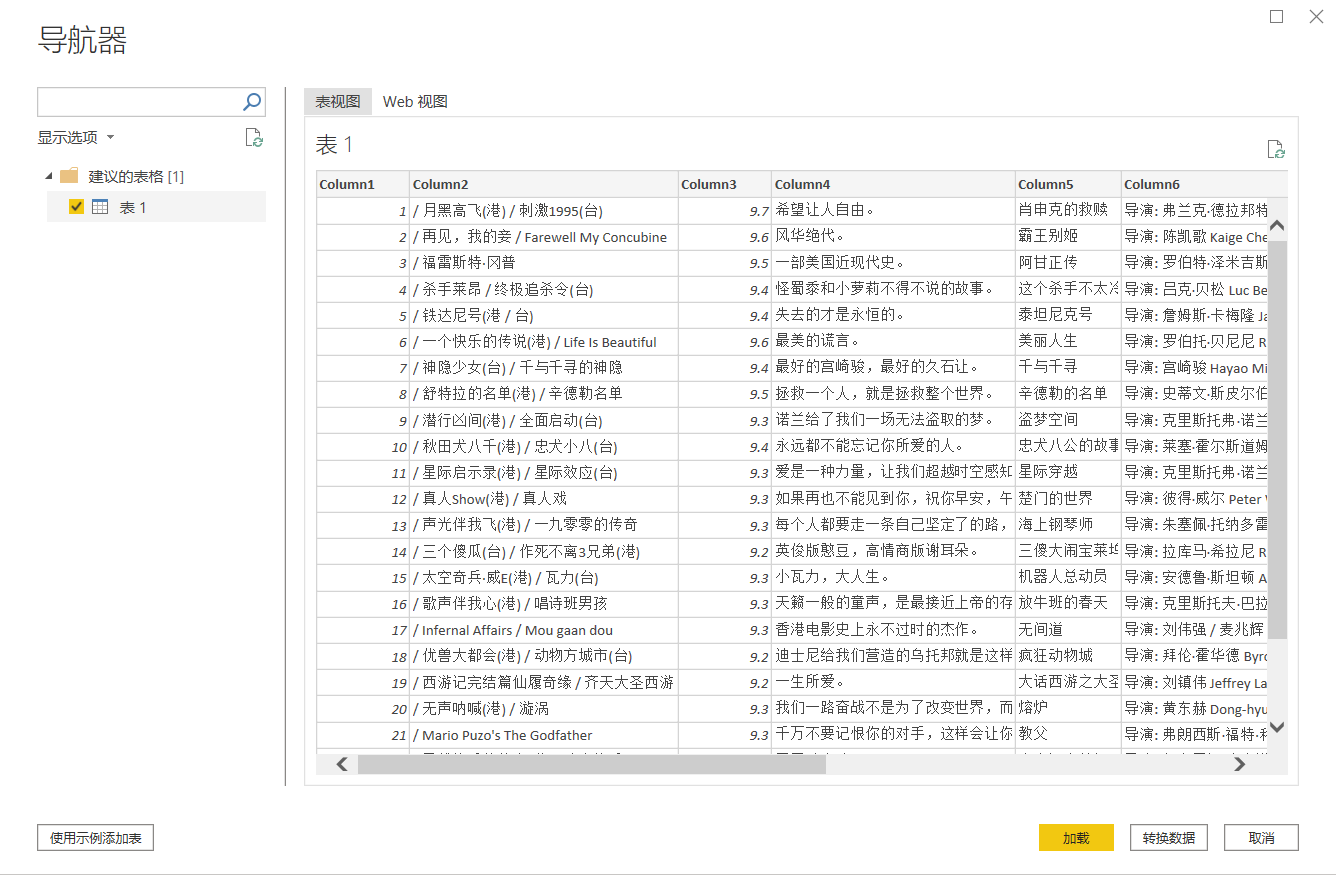
\includegraphics[width=0.9\textwidth]{figure/PowerBI/douban_advice_table.png}
    \caption{\textbf{自动识别出的建议的表格}}
    \label{fig:douban_advice_table}
\end{figure}

我们也可以使用``使用示例添加表''的功能去半自动地添加各列条目:只要输入前面几个数据,如电影名1,电影名2,系统会自动识别所要提取的数据类别,并自动地将网页中的剩余同类填充进来;但如果输入的数据没有规律,或者不是该网页中存在的数据,系统将无法识别。对于网页中不可见,但确实存在的信息,如电影的跳转详情页的获取,可以用类似的方法,将图片的URL链接复制到示例表里的各行,系统便会自动填充完整其他电影的跳转详情页链接。如\figref{fig:douban_example_table}所示。

\begin{figure}[htbp]
    \centering
    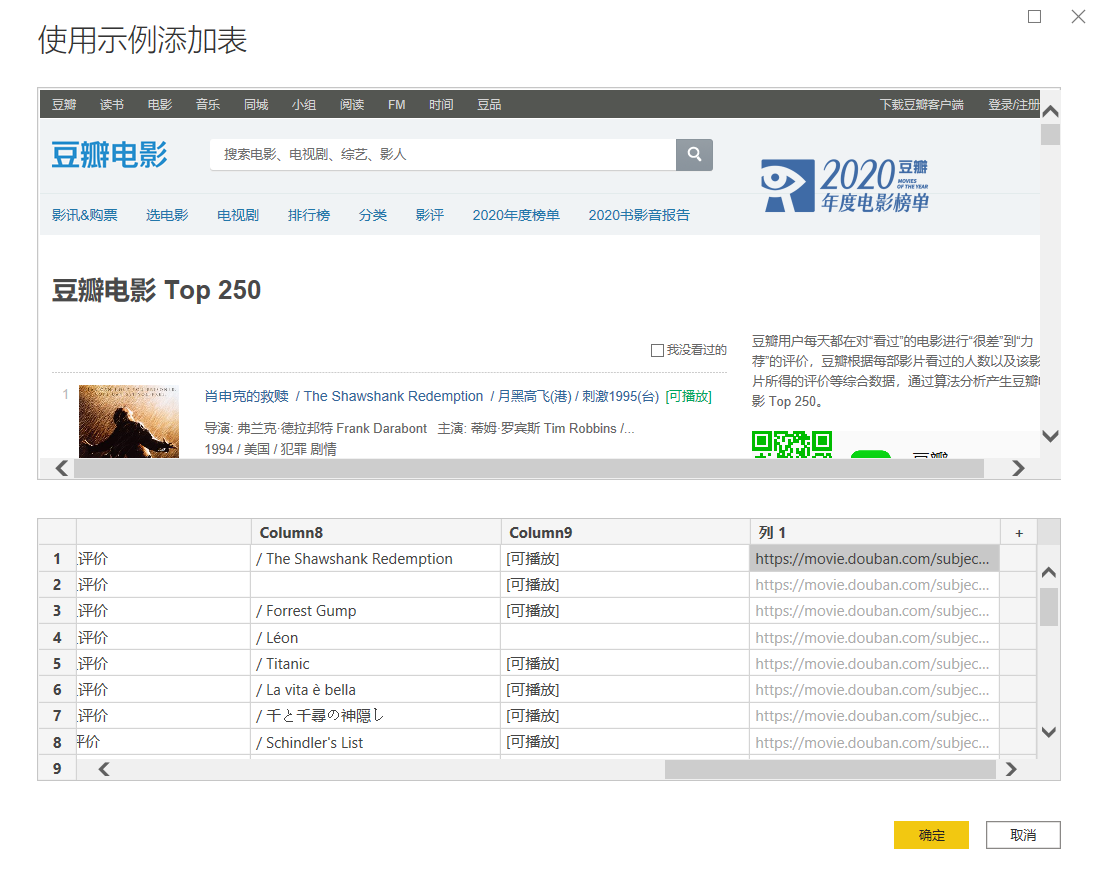
\includegraphics[width=0.9\textwidth]{figure/PowerBI/douban_example_table.png}
    \caption{\textbf{使用示例添加表添加电影详情页链接}}
    \label{fig:douban_example_table}
\end{figure}

然后就可以进入下个阶段:数据清洗。

\subsubsection{清洗第1页数据}

第1页提取的原始数据结构如\figref{fig:douban_raw_data_power_query}所示,在Power Query 编辑器中查看。

\begin{figure}[htbp]
    \centering
    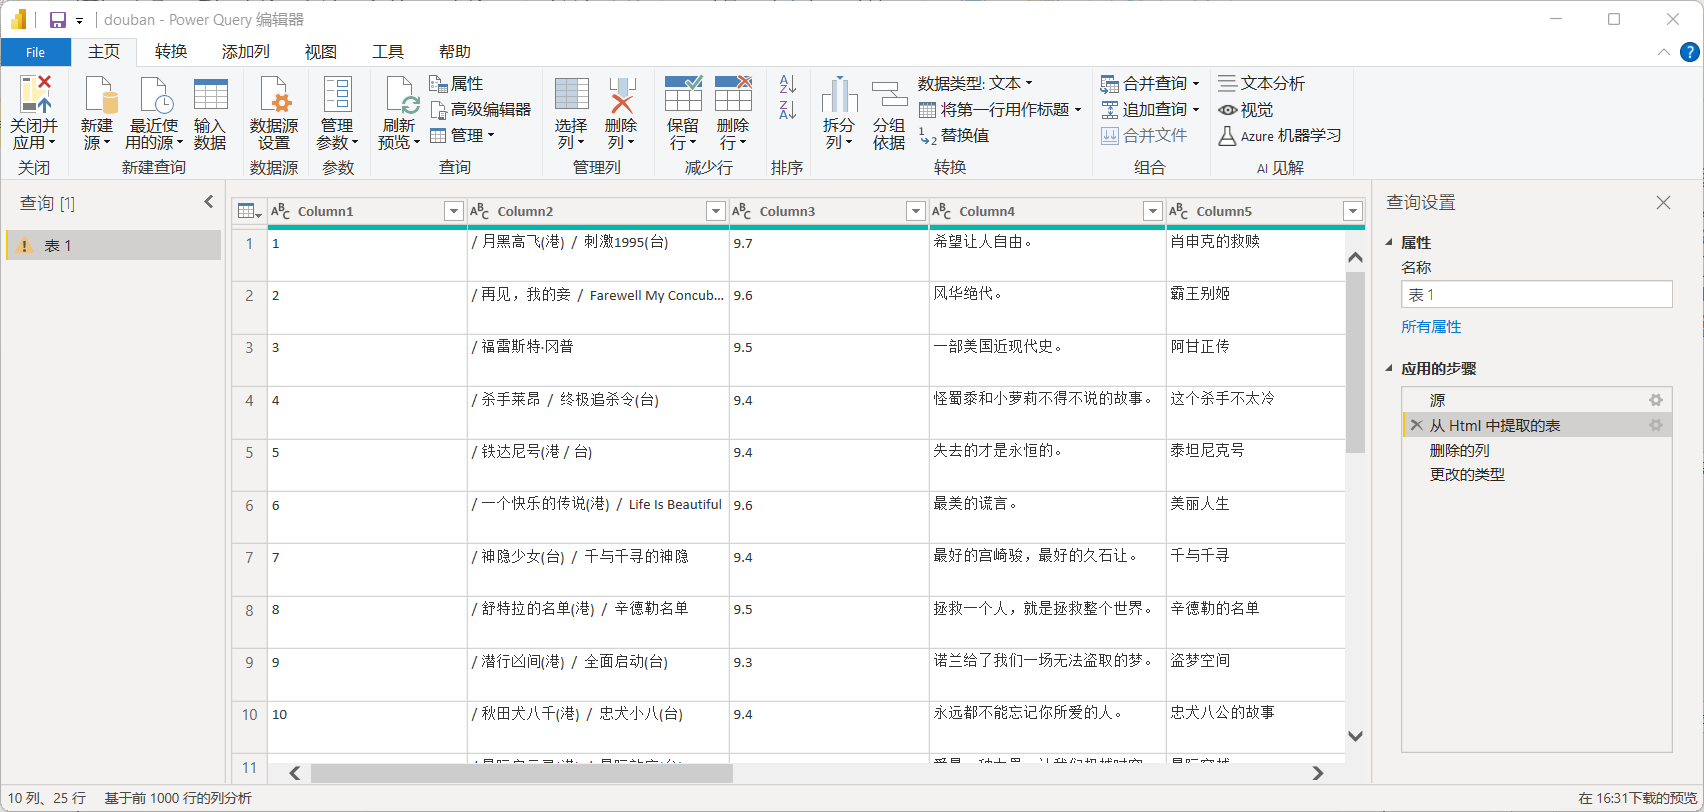
\includegraphics[width=0.9\textwidth]{figure/PowerBI/douban_raw_data_power_query.png}
    \caption{\textbf{提取的原始数据}}
    \label{fig:douban_raw_data_power_query}
\end{figure}

其实这个数据已经比较规范,部分列只需要修改数据类型、删除不必要的列,对部分列进行合并等操作。

对于电影名,有一些电影有别名和外文译名,我们可以对这些电影名进行合并:选择需要合并的列,点击``转换-合并列''即可进行合并。为了方便起见,此处仅保留在豆瓣电影中的第一个名称,删除其他含电影名的列。

对于多少人评价这一列,当前的内容为如``2406744人评价''的形式,其为一个文本类型,不方便对数据进行统计,因此我们在此可以使用替换值,将``人评价''替换为空值,这样就仅保留了数值,如\figref{fig:douban_data_replace}所示。

\begin{figure}[htbp]
    \centering
    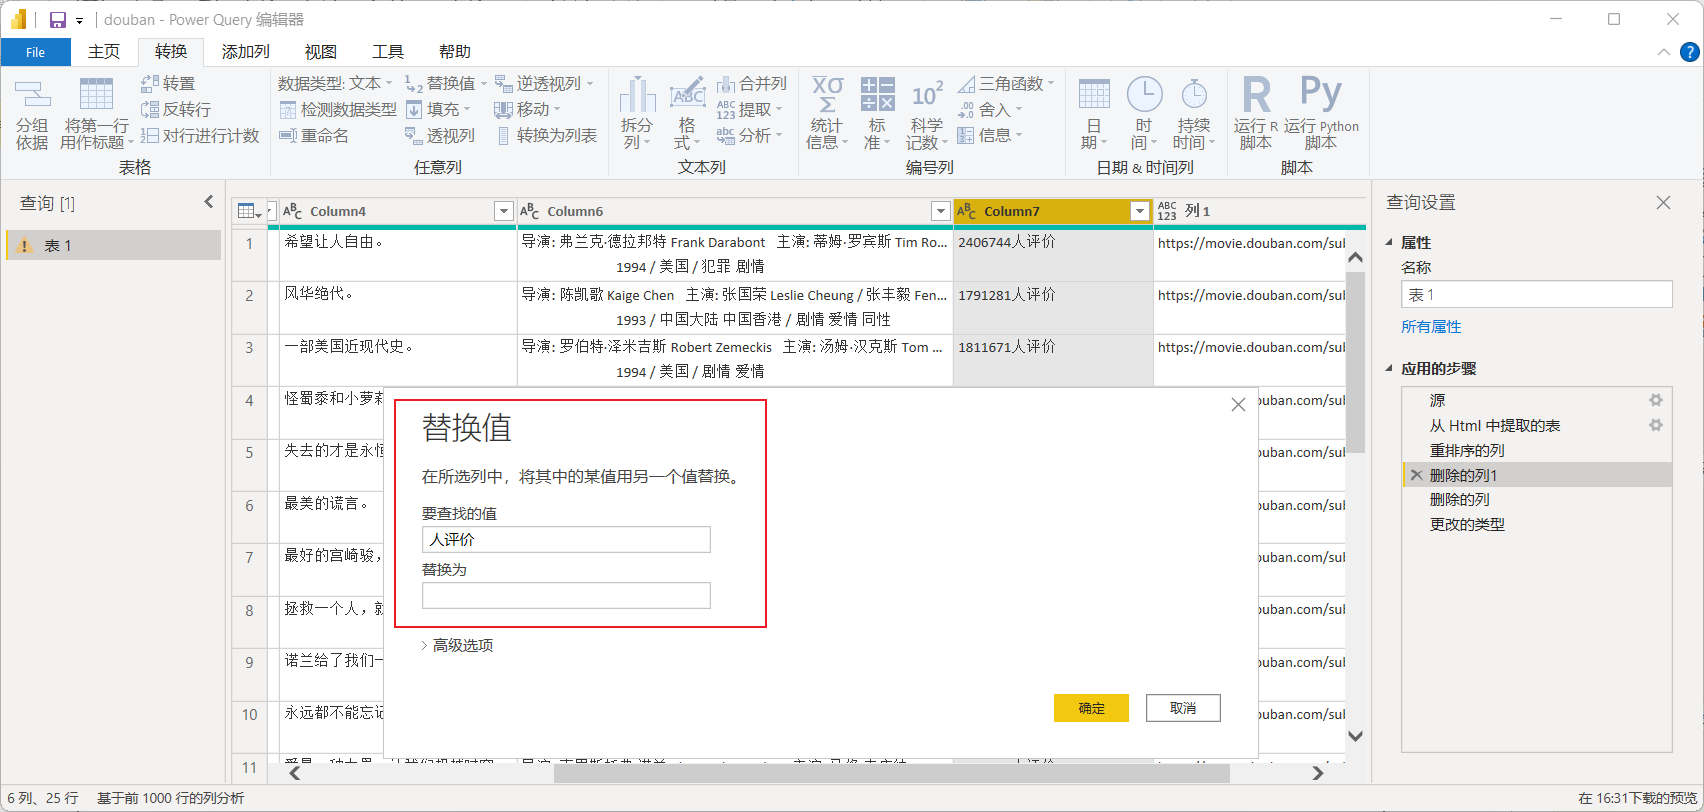
\includegraphics[width=0.9\textwidth]{figure/PowerBI/douban_data_replace.png}
    \caption{\textbf{替换``人评价'',保留数值}}
    \label{fig:douban_data_replace}
\end{figure}

于是,对于评分和评价人数可以进行数据类型转换,从文本类型分别转换为小数和整数。如\figref{fig:douban_data_type}所示中的操作。

\begin{figure}[htbp]
    \centering
    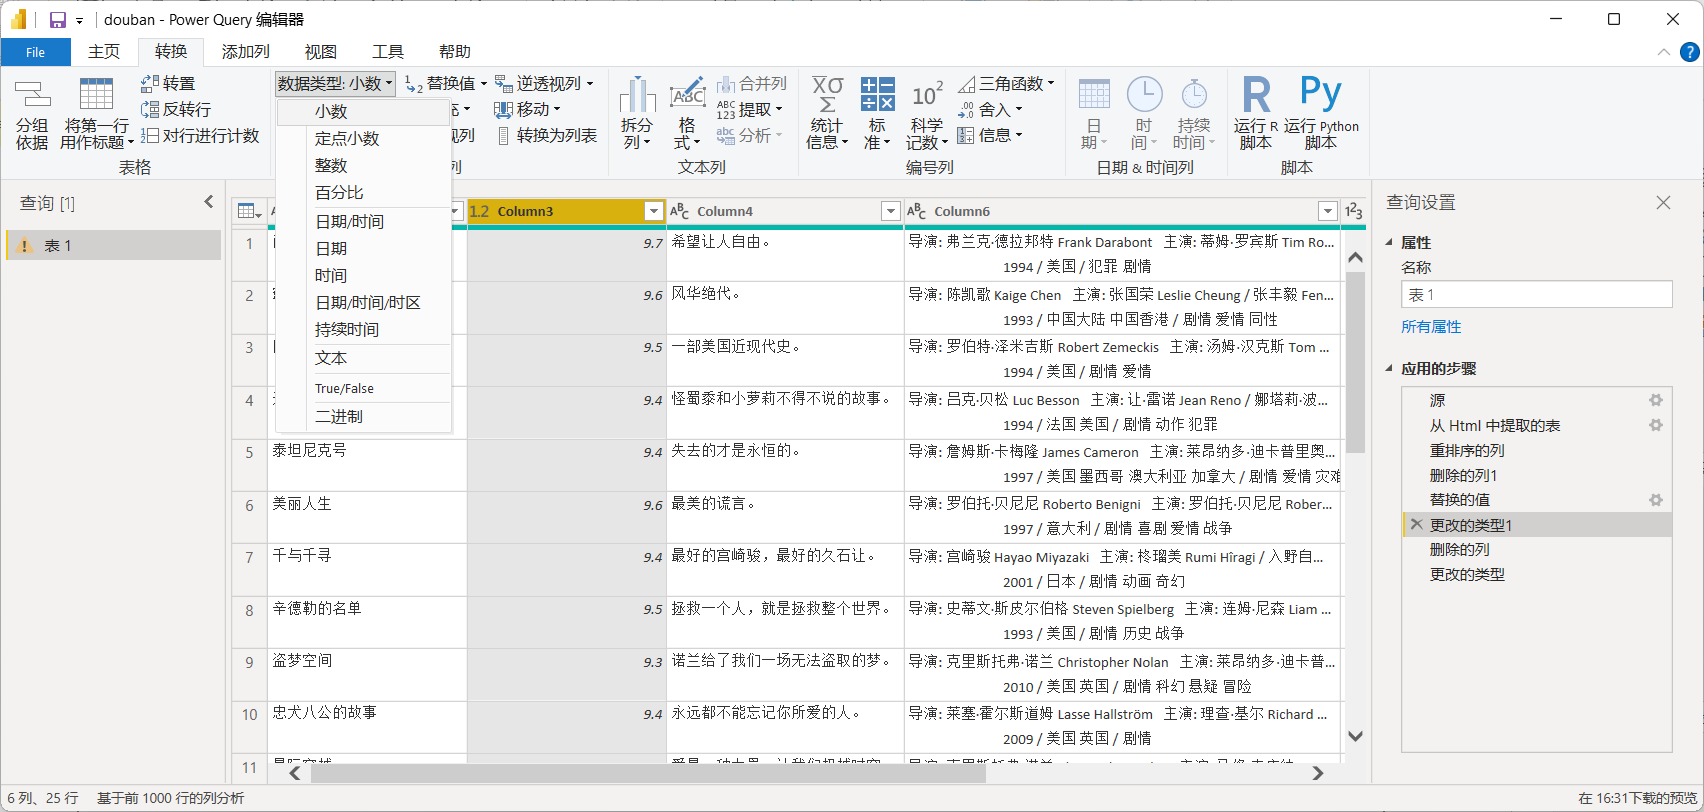
\includegraphics[width=0.9\textwidth]{figure/PowerBI/douban_data_type.png}
    \caption{\textbf{修改数据类型}}
    \label{fig:douban_data_type}
\end{figure}

另外,我们可以观察到电影信息列中将导演、主演、电影类型等信息放在了同一列,其不同类型的数据大多是通过``/''来分隔的。于是我们可以通过按分隔符拆分列来进行分隔提取。如\figref{fig:douban_split_data}所示选择``按分隔符拆分列''的操作。

\begin{figure}[htbp]
    \centering
    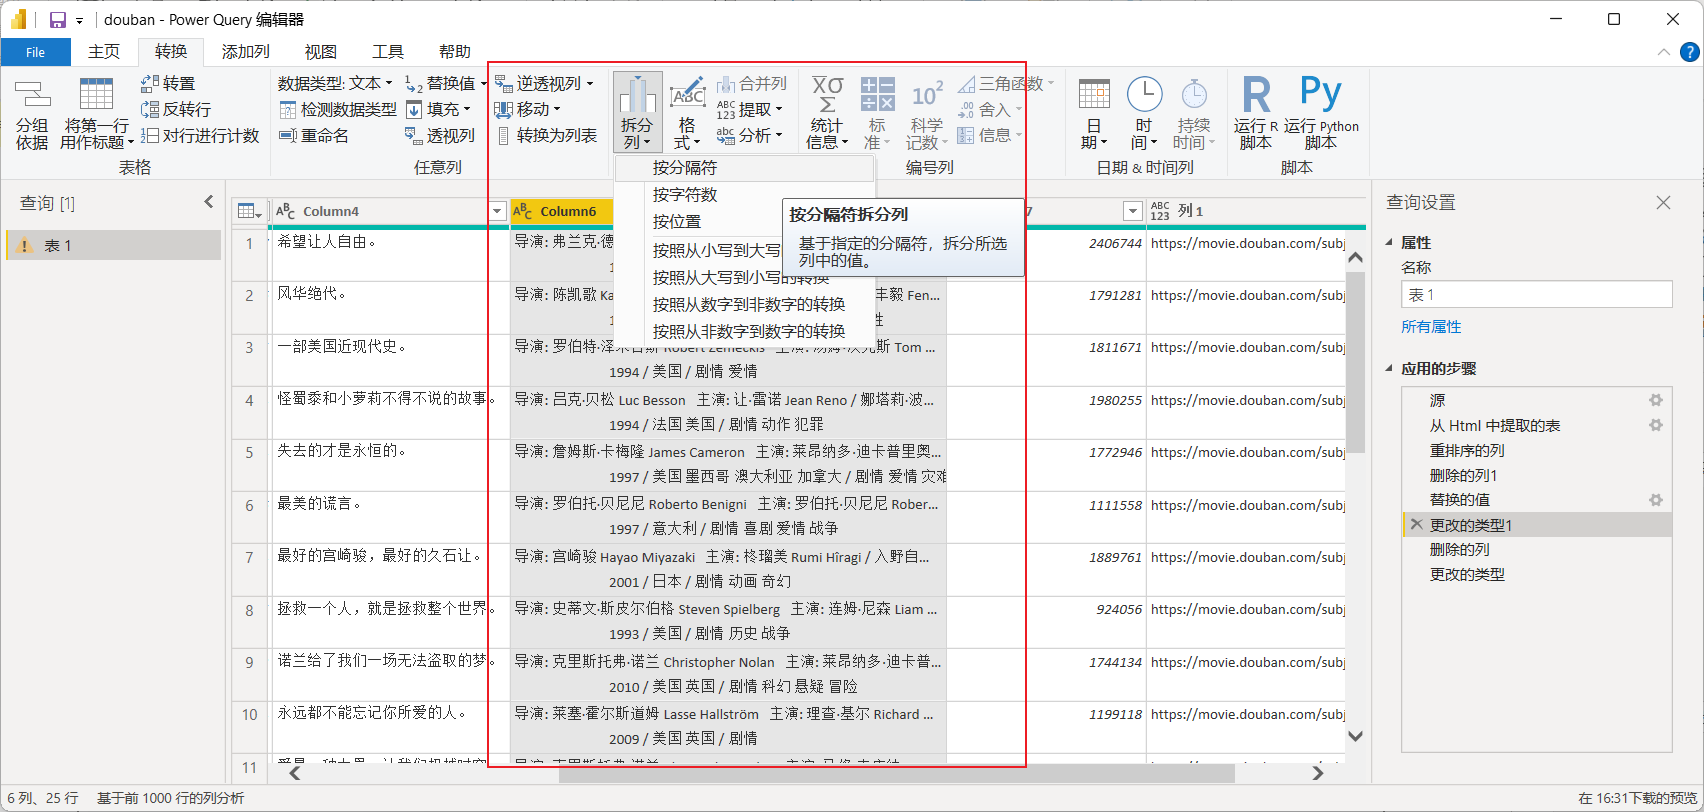
\includegraphics[width=0.9\textwidth]{figure/PowerBI/douban_split_data.png}
    \caption{\textbf{进入拆分数据操作}}
    \label{fig:douban_split_data}
\end{figure}

由于部分数据经分隔后有字段的缺省,没有对齐,但最后3个字段即年份、国家或地区、类型都是存在的,所以我们可以从右向左根据``/''逐列拆分。经过两次拆分后,对于年份信息是处于最后4个字符的,故可使用按照字符数(从右向左是5个字符)进行单独拆分。如\figref{fig:douban_split_from_right}所示为对类型和国家或地区的拆分。

\begin{figure}[htbp]
    \centering
    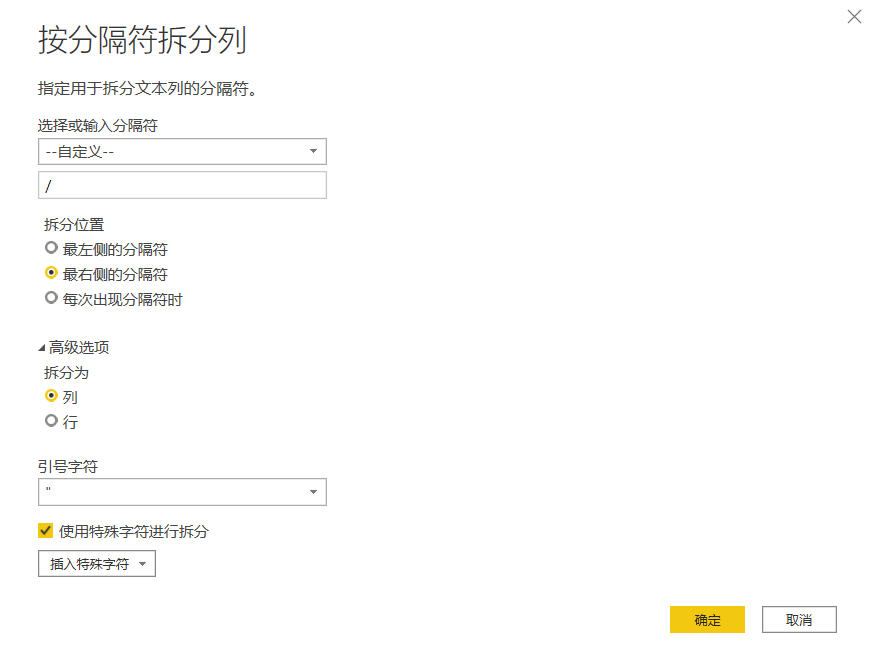
\includegraphics[width=0.5\textwidth]{figure/PowerBI/douban_split_from_right.png}
    \caption{\textbf{从右向左逐列拆分}}
    \label{fig:douban_split_from_right}
\end{figure}

如\figref{fig:douban_split_data_after}所示为拆分后的数据。

\begin{figure}[htbp]
    \centering
    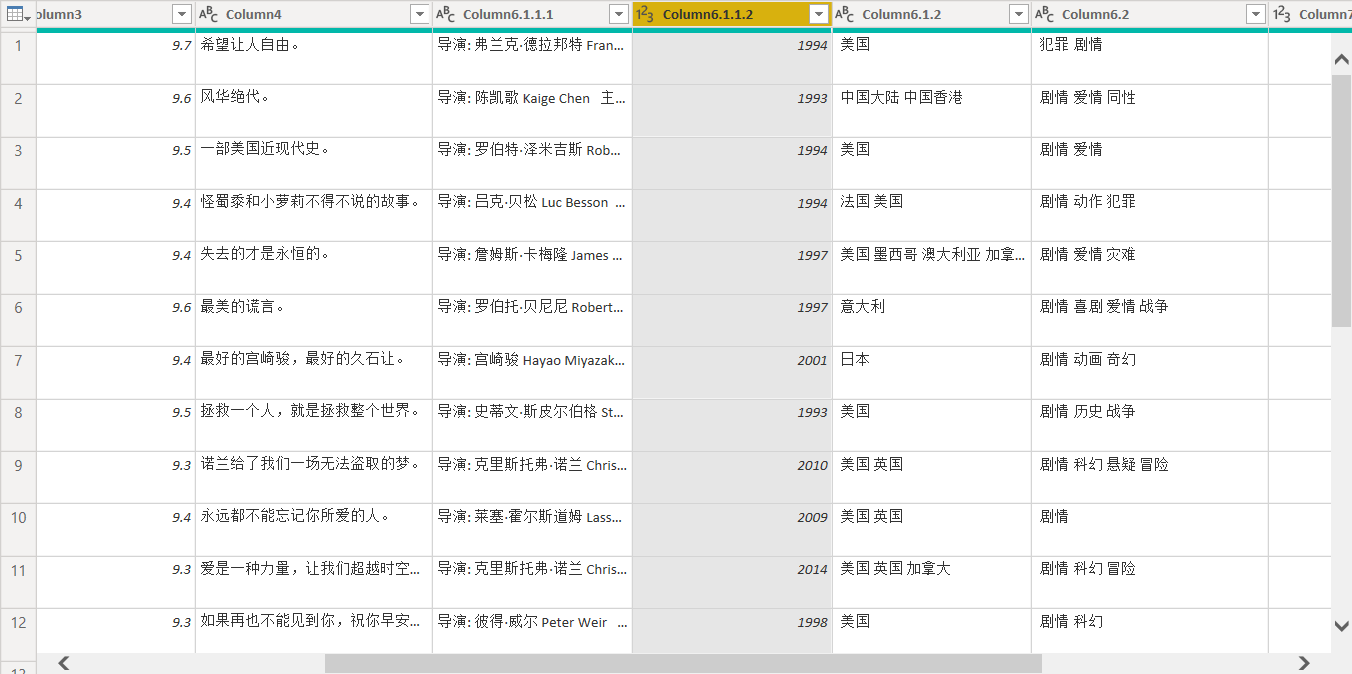
\includegraphics[width=0.9\textwidth]{figure/PowerBI/douban_split_data_after.png}
    \caption{\textbf{拆分后数据}}
    \label{fig:douban_split_data_after}
\end{figure}

然后,我们再次选取所需要的列进行数据分析,我在此保留了电影名、评分、评语、年份、国家或地区、类型、评分人数、详情页链接这8列,并将这8列的列名进行了对应的修改,如\figref{fig:douban_first_page_processed}所示。

\begin{figure}[htbp]
    \centering
    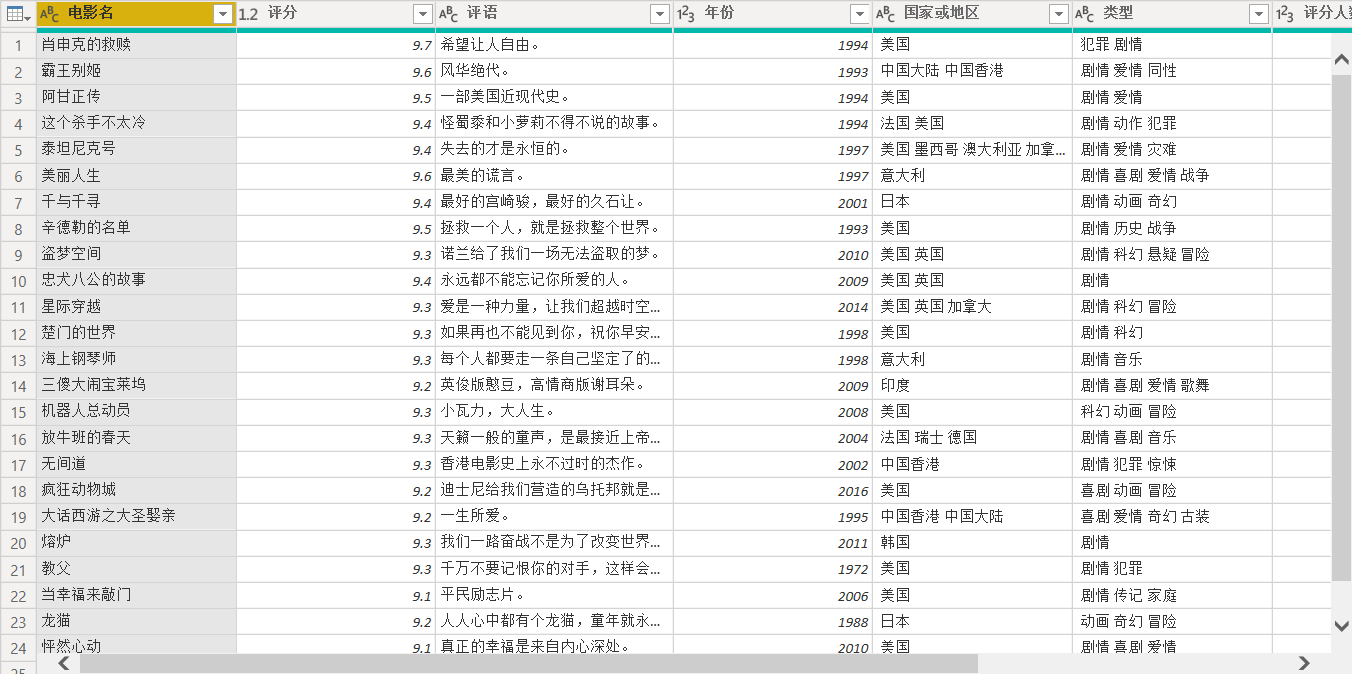
\includegraphics[width=0.9\textwidth]{figure/PowerBI/douban_first_page_processed.png}
    \caption{\textbf{第1页处理后数据}}
    \label{fig:douban_first_page_processed}
\end{figure}

至此,第1页的25条电影数据整理完成。

由于最终的目的是提取全部的250条数据,按以上相同的方法重复再做10次较为繁琐,我们考虑使用自定义函数批量提取多个网页数据。

\subsubsection{创建自定义函数}

在上一步已经整理好的第1页25条数据,已重命名该查询为``Top 25 电影'',右键单击该查询名,选择``创建函数'',如\figref{fig:douban_create_func}所示。

\begin{figure}[htbp]
    \centering
    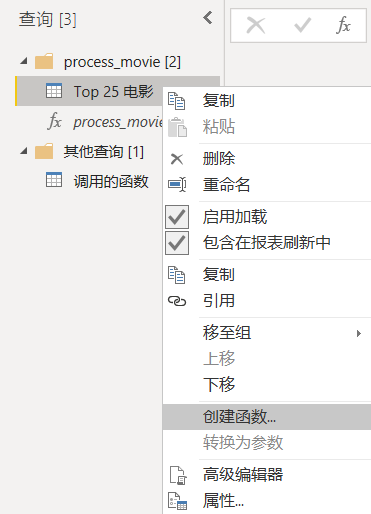
\includegraphics[width=0.4\textwidth]{figure/PowerBI/douban_create_func.png}
    \caption{\textbf{创建函数}}
    \label{fig:douban_create_func}
\end{figure}

如\figref{fig:douban_param_not_found}所示,弹出的窗口中会提示``未找到参数'',先不用理会,直接单击``创建''按钮,并输入函数名,此处将该函数命名为\verb|process_movie|。

\begin{figure}[htbp]
    \centering
    
\includegraphics[width=0.5\textwidth]{figure/PowerBI/douban_param_not_found.png}
    \caption{\textbf{未找到参数}}
    \label{fig:douban_param_not_found}
\end{figure}

然后单击该函数,在编辑栏中(如没有,需要先点击``视图'',勾选出``编辑栏'')手动更改代码,将前两行代码更改如下,如\figref{fig:douban_func_code}所示。


\begin{minted}
[
frame=lines,
framesep=2mm,
baselinestretch=1.2,
fontsize=\footnotesize,
linenos
]{js}
= (x as text) => let
        网址 = "https://movie.douban.com/top250?start="&x,
        源 = Web.BrowserContents(网址),
\end{minted}

\begin{figure}[htbp]
    \centering
    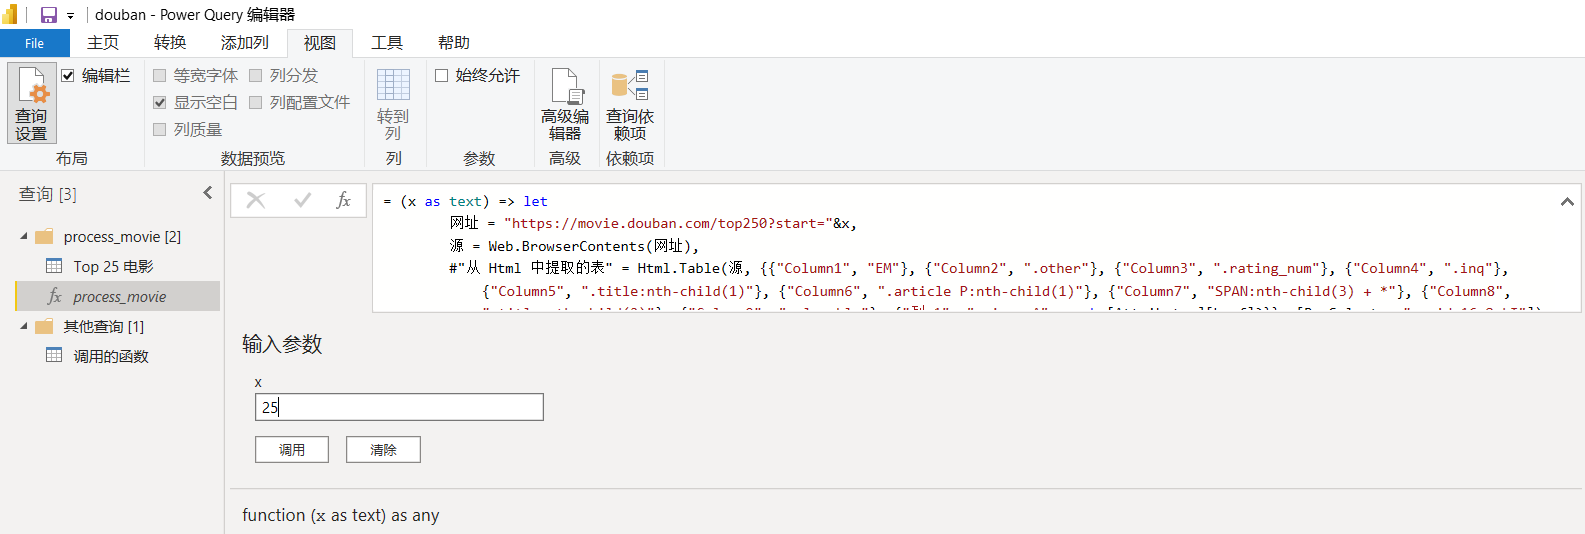
\includegraphics[width=0.9\textwidth]{figure/PowerBI/douban_func_code.png}
    \caption{\textbf{修改自定义函数代码}}
    \label{fig:douban_func_code}
\end{figure}

此处就是将网址分为了两个部分,如第1页的地址为:\url{https://movie.douban.com/top250?start=0},将第一部分\url{https://movie.douban.com/top250?start=}作为常量文本保持不变,而最后一个数字,变为参数\verb|x|,二者组合到一起作为一个完整的网址,然后便只需将不同的数字赋给\verb|x|,就可以提取该页的数据。

开头的\verb|= (x as text) =>|表示该自定义函数的参数为\verb|x|,参数类型为\verb|text|,创建好的自定义函数下方,也出现了输入参数的输入框。

这样便创建好了一个自定义函数。如果在输入参数框中输入25,单击``调用''按钮,即可获得第2页的电影内容,因为该自定义函数包含了第1页中数据清洗的所有步骤。下面可利用该自定义函数一次性提取多页的数据。

\subsubsection{构建参数列表}

通过上述对网址URL的分析,这10页网址最后一个数字为0、25、50……225,所以需要构造这个等差数列作为自定义函数的参数。

在Power Query中,选择``主页-新建源-空查询'',如\figref{fig:douban_new_query}所示。然后在编辑栏中输入:

\begin{figure}[htbp]
    \centering
    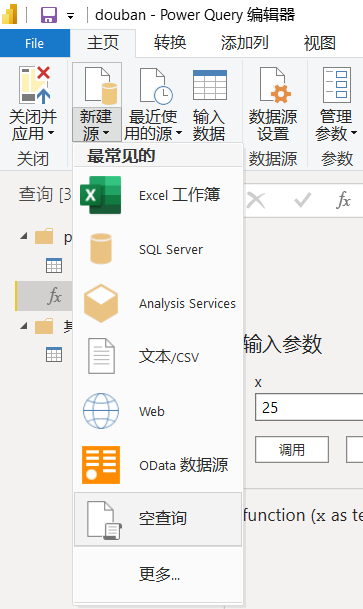
\includegraphics[width=0.4\textwidth]{figure/PowerBI/douban_new_query.png}
    \caption{\textbf{新建空查询}}
    \label{fig:douban_new_query}
\end{figure}

\begin{minted}
[
frame=lines,
framesep=2mm,
baselinestretch=1.2,
fontsize=\footnotesize,
linenos
]{js}
= List.Numbers(0, 10, 25)
\end{minted}

即可得到该参数列表,如\figref{fig:douban_new_list}所示。

\begin{figure}[htbp]
    \centering
    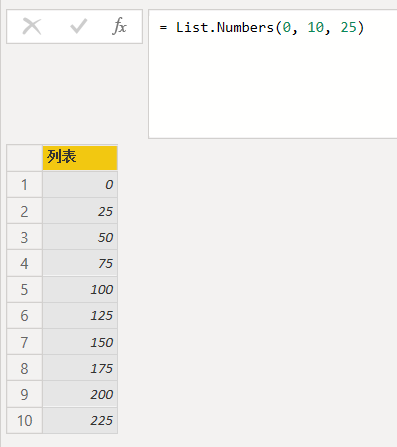
\includegraphics[width=0.4\textwidth]{figure/PowerBI/douban_new_list.png}
    \caption{\textbf{生成参数列表}}
    \label{fig:douban_new_list}
\end{figure}

其中,\verb|List.Numbers(0, 10, 25)|表示从0开始,后续的数字递增25,生成10个数字。选择``转换-转换到表'',即可将这一组数字转换为Power Query中的一个表,在此将该表重命名为``参数页表''。

\subsubsection{批量提取多个网页数据}

在上面生成的参数页表中,注意将该列的值指定为``文本'',然后在``添加列''中选择``调用自定义函数'',在弹出的窗口中,直接选择已经建立好的自定义函数,参数选择上一步建好的参数列,如\figref{fig:douban_call_param}所示。

\begin{figure}[htbp]
    \centering
    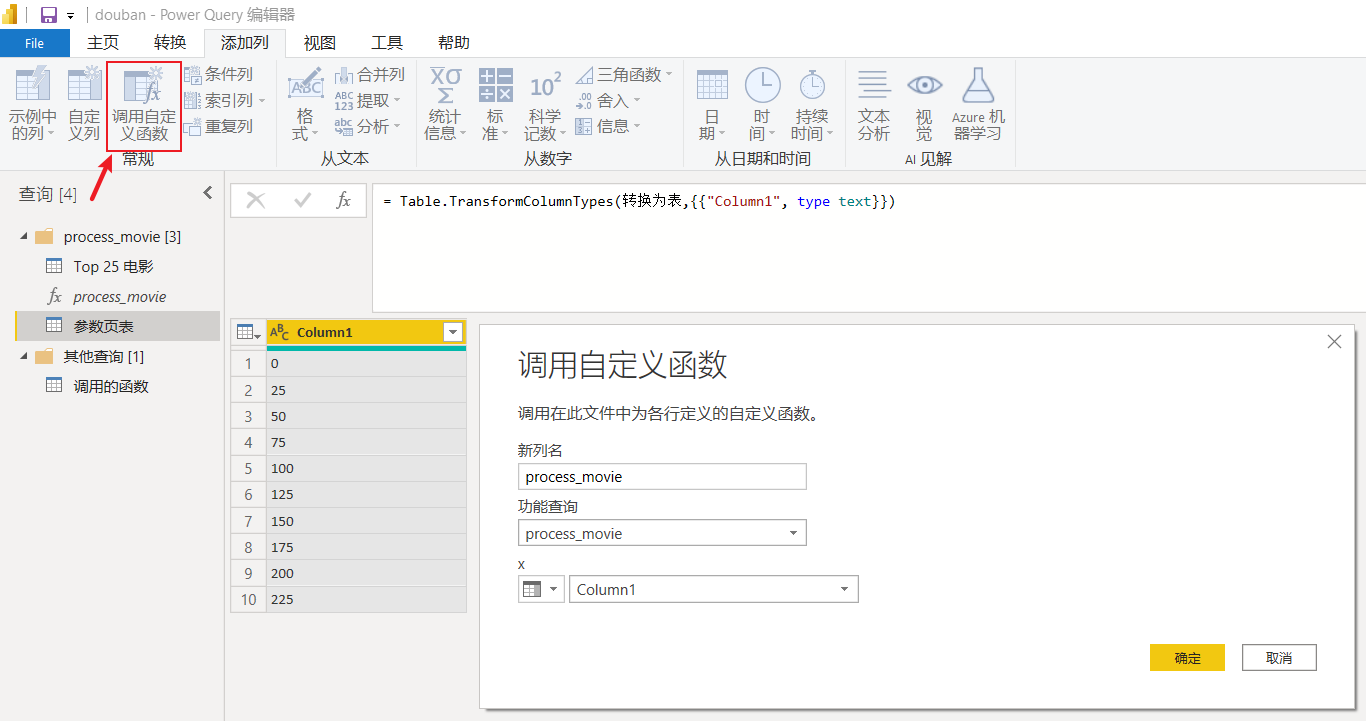
\includegraphics[width=0.9\textwidth]{figure/PowerBI/douban_call_param.png}
    \caption{\textbf{调用自定义函数}}
    \label{fig:douban_call_param}
\end{figure}

然后展开新生成的自定义列,即可得到全部的10页Top 250的电影数据,稍加整理,删除不必要的列,重命名列,并添加一个索引列,该表命名为``Top 250 电影信息表'',于是便完成了数据获取和整理过程,关闭并上载到Power BI中,最终数据如\figref{fig:douban_top250_fetched}所示。

\begin{figure}[htbp]
    \centering
    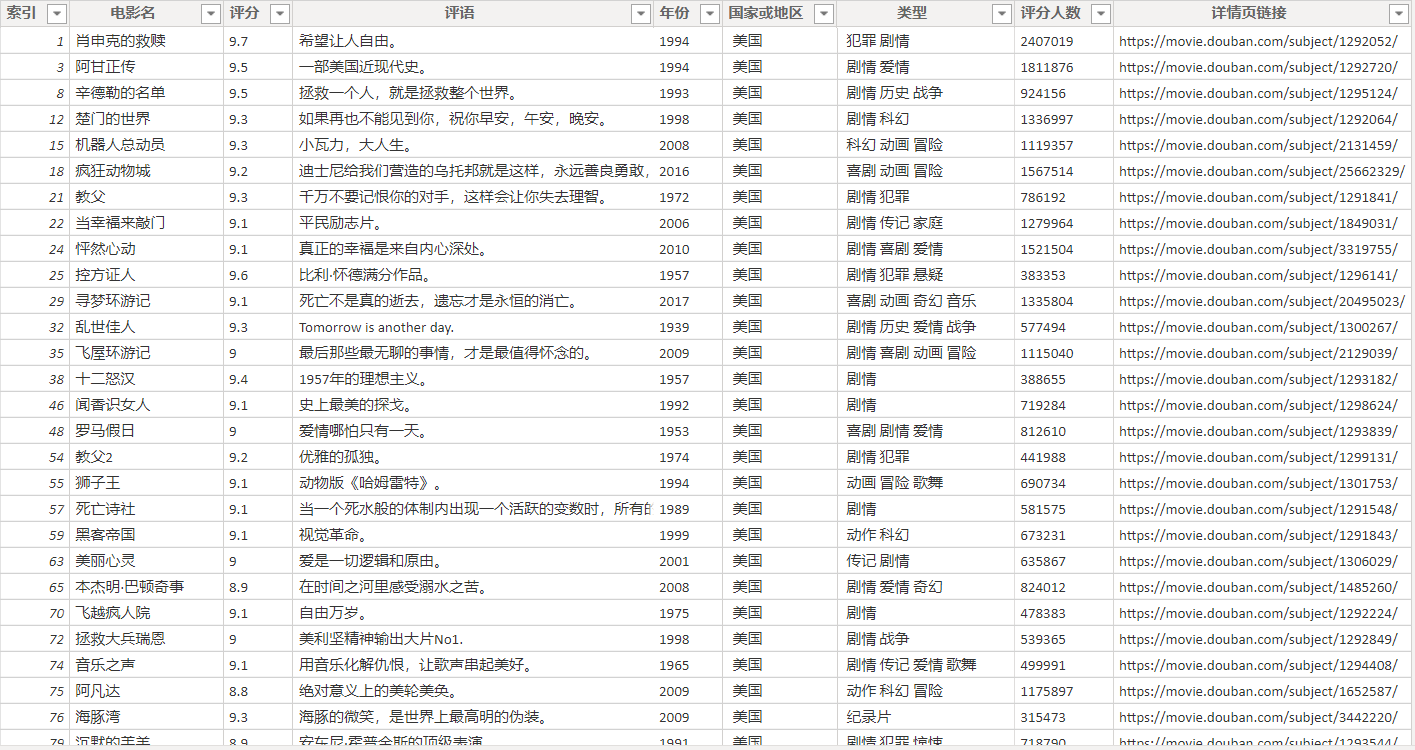
\includegraphics[width=0.9\textwidth]{figure/PowerBI/douban_top250_fetched.png}
    \caption{\textbf{完成豆瓣电影Top 250 的数据获取}}
    \label{fig:douban_top250_fetched}
\end{figure}

% \section{数据建模}

% 需要分析的数据通常并不是只有一张表,为了分析的需要,也要将表分为事实表和维度表,这些不同的表,需要协同配合才能更好地使用,协同配合依靠表与表之间的逻辑关系,这个建立关系的过程就称为数据建模。

% 一个良好的数据模型是数据分析的基础,也是一个良好的可视化报告的基础,建立一个良好的模型,可以更简单地实现分析的目的。

% 在Power Query中清洗后的数据上载进来后,根据需要添加维度表、度量表或者计算列,

% \begin{minted}
% [
% frame=lines,
% framesep=2mm,
% baselinestretch=1.2,
% fontsize=\footnotesize,
% linenos
% ]{js}
% 豆瓣评分 = MAX('Top 250 电影信息表'[评分])
% 电影数量 = COUNTROWS('Top 250 电影信息表')

% 评分排名 = RANK(ALL('电影名表'),[豆瓣评分])
% \end{minted}

\subsection{数据可视化}

经过了上述的数据获取、整理和清洗操作,接下来可将数据结果以图表的形式来展现,让数据更易于理解。

\subsubsection{制作电影信息列表}

在报表视图,选择加载好的``Top 250 电影信息表'',勾选所需的数据字段后,会自动生成列表,如\figref{fig:douban_movie_list}所示。

\begin{figure}[htbp]
    \centering
    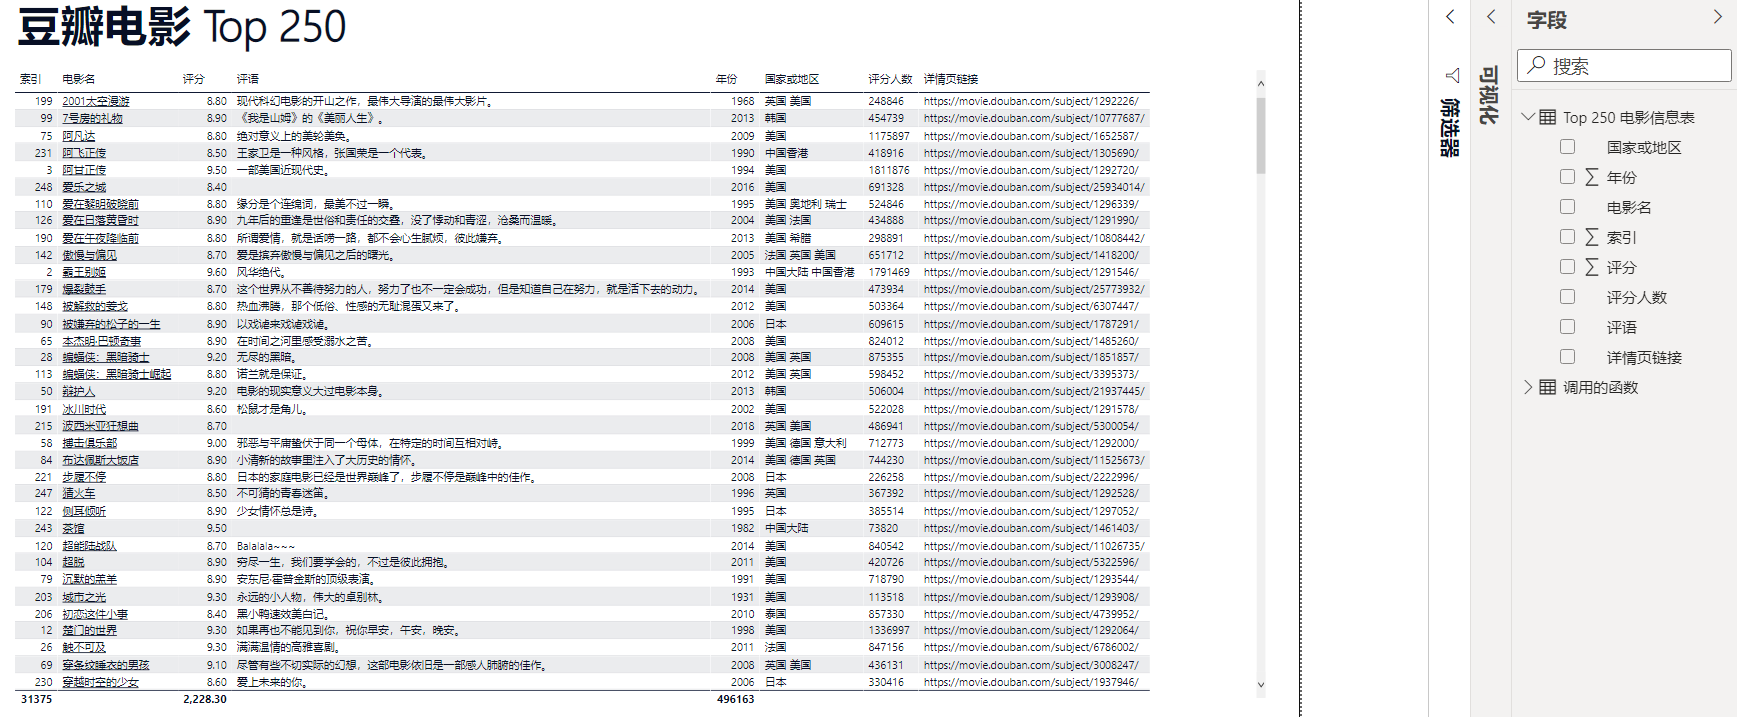
\includegraphics[width=0.9\textwidth]{figure/PowerBI/douban_movie_list.png}
    \caption{\textbf{电影信息列表展示}}
    \label{fig:douban_movie_list}
\end{figure}

我们可以利用到电影详情页的链接地址,设置从电影名列到详情页的URL跳转,如\figref{fig:douban_select_url}中,在可视化区域栏中的格式页中的条件格式区,先选择了电影名字段,并打开Web URL选项。之后,在弹出的窗口中的``依据为字段''中,选择``第一个 详情页链接'',即可在列表中点击电影名后跳转到系统浏览器中的电影详情页,电影名字段也显示了下划线。

\begin{figure}[htbp]
    \centering
    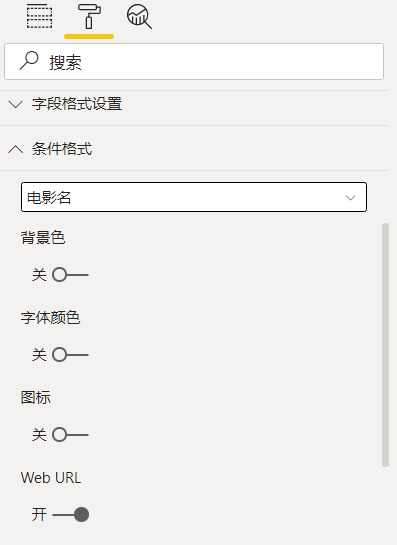
\includegraphics[width=0.5\textwidth]{figure/PowerBI/douban_select_url.png}
    \caption{\textbf{打开Web URL}}
    \label{fig:douban_select_url}
\end{figure}

\subsubsection{制作电影评分和排名表}

这里我们将为评分情况作出分析图表:电影名和评分的条形图、评分和年份之间的折线图。

对于电影名和评分的条形图的绘制,勾选电影名和评分两个字段,其中注意评分的数据格式需设置为定点小数。在可视化区域,选择``堆积条形图'',分别设置轴中的字段为``电影名'',值为``评分的平均值''(平均值是做了数据的汇总,防止有同名电影的情况,虽然并不存在)。在格式区,可以设置打开数据标签,则在条形图的右侧会显示出具体的评分,还可以开启缩放滑块,让X轴坐标不一定从0开始。如\figref{fig:douban_score_movie_name}中所示。

\begin{figure}[htbp]
    \centering
    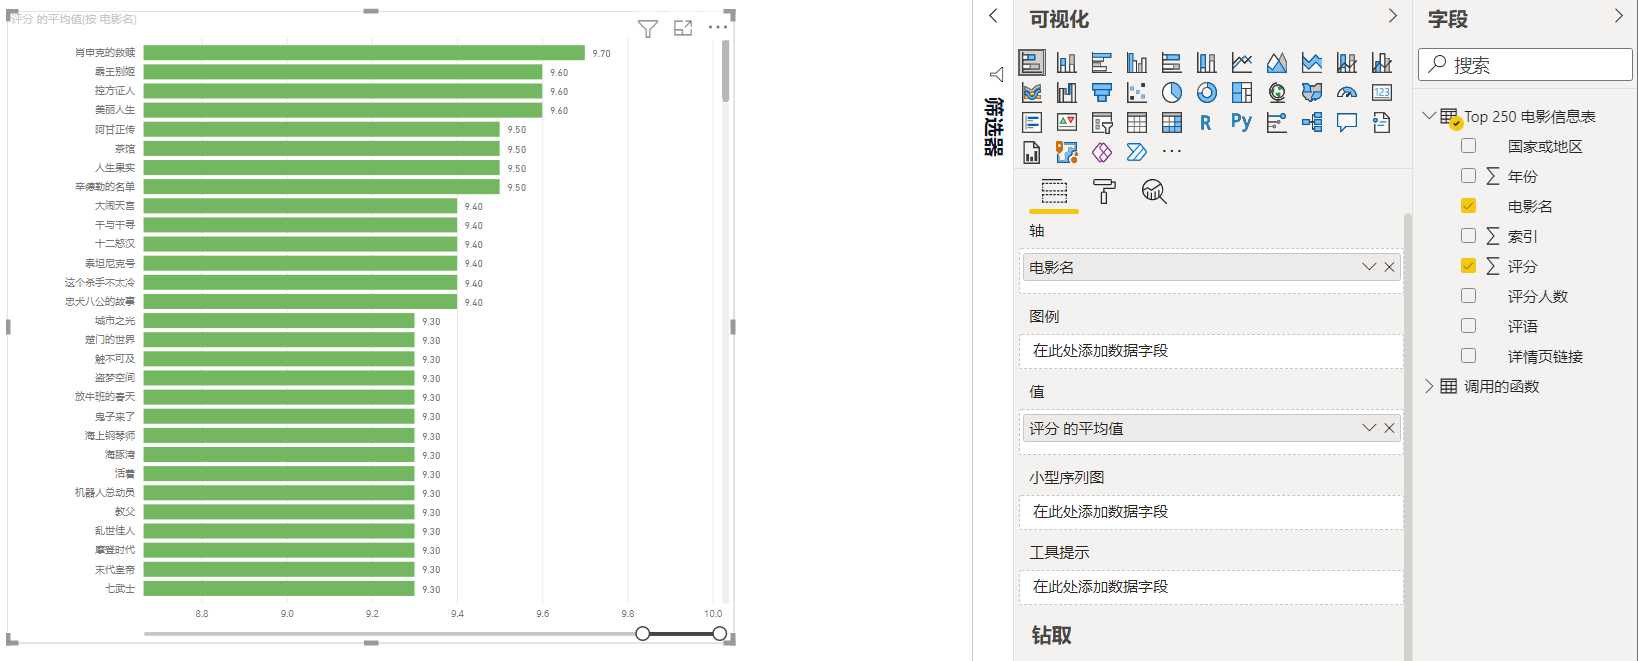
\includegraphics[width=0.9\textwidth]{figure/PowerBI/douban_score_movie_name.png}
    \caption{\textbf{电影名和评分的条形图}}
    \label{fig:douban_score_movie_name}
\end{figure}

对于评分和年份之间的折线图的绘制,勾选年份和评分两个字段,其中注意年份的数据格式需设置为整数形,在可视化区域,选择``折线图''后即可。同理设置轴与值的字段,并可以在格式区打开数据标签和开启缩放模块。如\figref{fig:douban_score_year}中所示。

\begin{figure}[htbp]
    \centering
    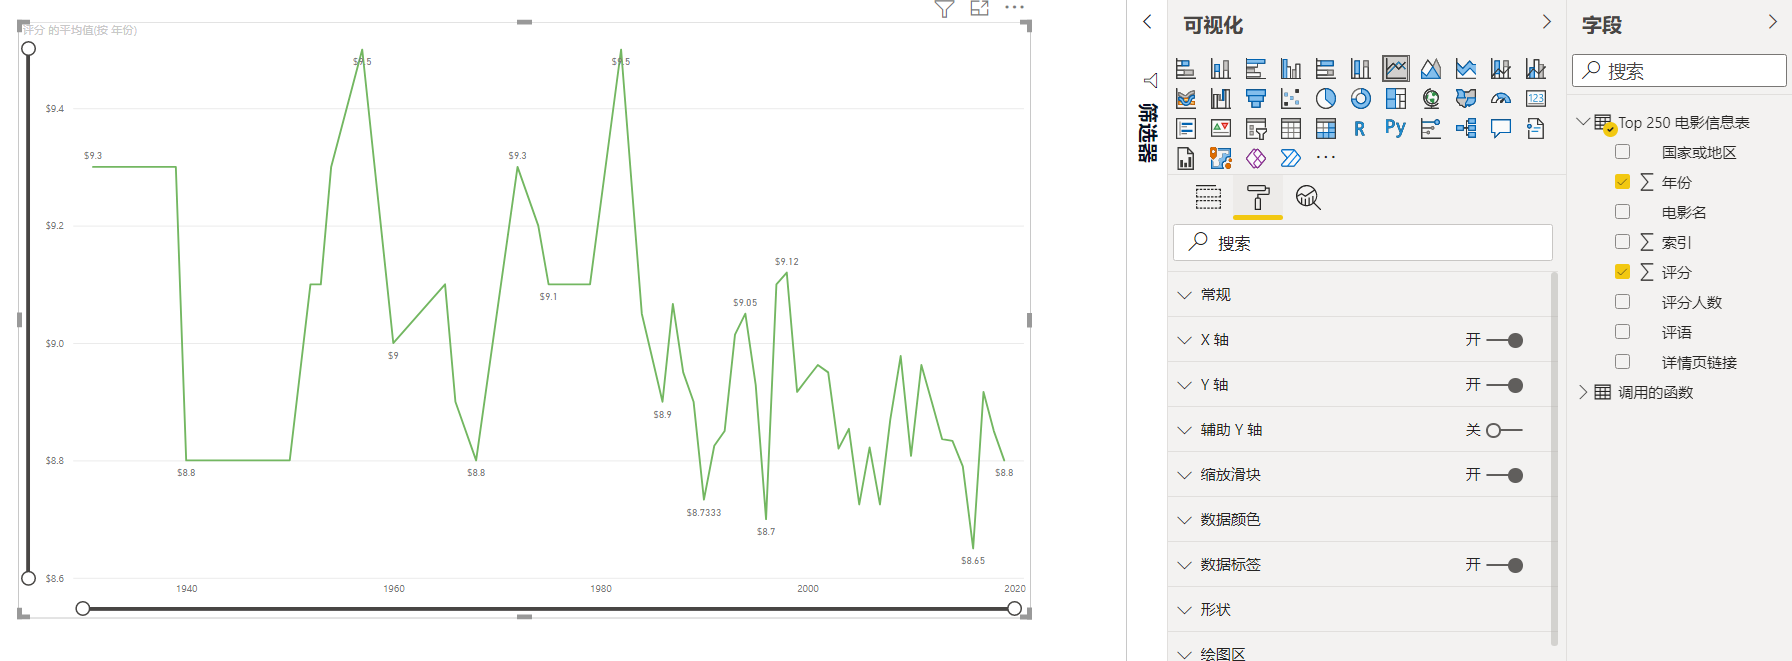
\includegraphics[width=0.9\textwidth]{figure/PowerBI/douban_score_year.png}
    \caption{\textbf{评分和年份之间的折线图}}
    \label{fig:douban_score_year}
\end{figure}

Power BI中还提供了一些分析工具,如我们可以在可视化区域中的分析页中,添加趋势线,见\figref{fig:douban_score_year_trend}所示。我们还能对数据进行预测(前提是数据字段均非空)。

\begin{figure}[htbp]
    \centering
    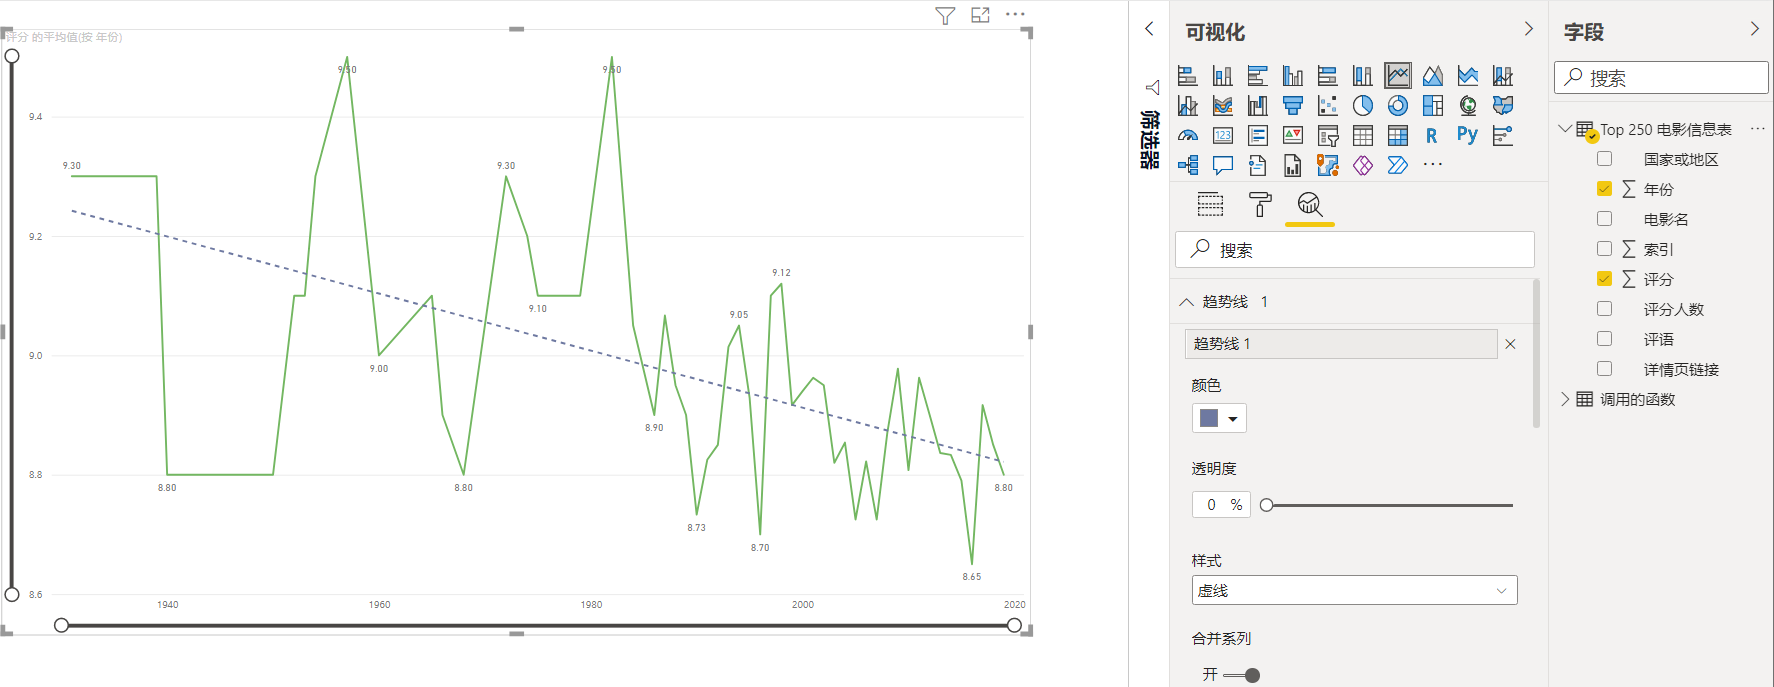
\includegraphics[width=0.9\textwidth]{figure/PowerBI/douban_score_year_trend.png}
    \caption{\textbf{添加趋势线}}
    \label{fig:douban_score_year_trend}
\end{figure}

\subsection{发布报表}

前几步生成的Power BI报告,不仅可以在本机查看,还可以更方便地发布到Web上与他人分享。

在Power BI的功能区,点击``发布'',可选择``我的工作区'',发布报表,发布成功后即可在网页上浏览报表。如\figref{fig:powerbi_publish}所示,选择``在Power BI中打开''便会跳转至网页浏览器,保存该网页链接便能在移动端等各设备随时随地查看,并可以和其他人方便地分享报表。

\begin{figure}[htbp]
    \centering
    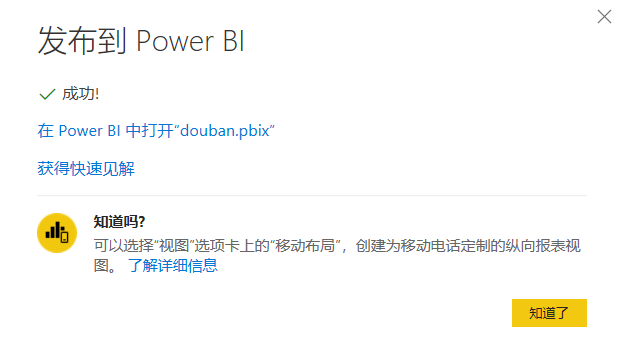
\includegraphics[width=0.5\textwidth]{figure/PowerBI/powerbi_publish.png}
    \caption{\textbf{发布 Power BI 报表}}
    \label{fig:powerbi_publish}
\end{figure}

以上就是使用Power BI进行数据分析的基本步骤,从数据获取到数据可视化以及最后的报告分享,我们对Power BI的使用有了一个较为完整的认识。Power BI还有许多功能,如使用Power BI进行数据建模、DAX数据分析语言等等,我们可以通过查阅官方文档、网络上的各种教程等方式进一步深入学习。